% \tocless
\section{Empirical Applications}\label{sec:empirical}

We run synthetic experiments on multiple real data sets to study our solutions in Sections \ref{sec:model} and \ref{sec:sequential-experiment}.
\footnote{Our code is available at \protect\url{https://github.com/ruoxuanxiong/staggered_rollout_design}.}
  First, we describe the data sets that we study from multiple domains in Section \ref{subsec:data-description}.
Next, in Section \ref{subsec:empirical-fixed-sample-size}, we show that for non-adaptive experiments, our solutions from Section \ref{subsec:result-carryover} require less than 50\% of the sample size to achieve the same treatment effect estimation error as the benchmark designs. For adaptive experiments, in Section \ref{subsec:empirical-sequential}, we show that our adaptive design from PGAE can improve the precision of treatment effect estimation by more than 20\%, on top of the improvements obtained by our non-adaptive designs. 

% \tocless
\subsection{Data Descriptions}\label{subsec:data-description}
Our synthetic experiments are run on four different data sets. The first one, MarketScan Research Databases, is used for the empirical results of this section. As robustness checks, the same results are shown on the remaining three data sets in Section \ref{subsec:description-data-sets}.

\paragraph{MarketScan research databases.} 
These databases contain inpatient and outpatient claim records. Focusing on influenza as the primary diagnosis, there are 21,277 inpatient admissions versus 9,678,572 outpatient visits in the databases. We denote all of these as influenza visits. Our outcome variables are monthly \emph{flu visit occurrence rates} per Metropolitan Statistical Area (MSA) and per thousand patients, which is defined as the ratio of the number of influenza visits among all enrolled patients times $1,000$ for the given month in a given MSA. Moreover, our analysis focuses on the flu peak seasons that are defined as October to April of the next year. We focus on the period from October 2007 to April 2015 as the databases have few observations outside this period. This leaves us with a panel of $185$ MSAs over $56$ months.
See Section \ref{subsec:description-data-sets} for more details.



\paragraph{Other data sets.} The three additional data sets, as described in Section \ref{subsec:description-data-sets}, are home medical visits in 61 cities over 144 weeks, grocery store transactions for 7,130 households over 97 weeks, and Lending Club loans for 956 geographic areas in the US over 139 months.

\subsection{Non-Adaptive Experiments}\label{subsec:empirical-fixed-sample-size}
First, in Section \ref{subsec:experiment-setup}, we discuss the setup of synthetic experiments and evaluation criteria, and then present the results in Section \ref{subsec:fixed-sample-empirical-results}. 

\subsubsection{Setup}\label{subsec:experiment-setup}
\texttt{} \\
Here, we first introduce the benchmark designs as well as different versions of our solution, depending on the specifications of the estimator. Then we explain how the synthetic experiment and treatment effect are generated, and then discuss the evaluation metrics that are used.

	{\bf Treatment designs.}
	We consider the following treatment designs. Illustrations of these designs in Figure \ref{fig:various-optimal-design} of Section \ref{sec:model} can facilitate the reading.
	\begin{enumerate}
		\item \emph{Benchmark treatment designs:}
		\begin{enumerate}
		\item $Z_{\FF}$ (fifty-fifty): $Z_{\FF}$ has 50\% control and 50\% treated units at every time period. More precisely, $Z_{\FF}$ is a rounded solution when starting with $\omega_s = 0$ for all $s$.
			\item $Z_{\BA}$ (before-after): $Z_{\BA}$ has all units in the control state before halftime and all units in the treatment state after halftime. More precisely, $Z_{\BA}$ is a rounded solution that starts with $\omega_s = -1$ for $s < (T+1)/2$ and equals to $\omega_s = 1$ for $s \geq (T+1)/2$.
			\item $Z_{\FFBA}$ (fifty-fifty with before-after): $Z_{\FFBA}$ has all units in the control state before halftime and half of the units in the treatment state after halftime. That is, $Z_{\FFBA}$ is a rounded solution that starts with $\omega_s = -1$ for $s < (T+1)/2$ and has $\omega_s = 0$ for $s \geq (T+1)/2$. $Z_\FFBA$ combines $Z_\FF$ and $Z_\BA$, and has the simultaneous treatment adoption pattern.
		\end{enumerate}
		
		\item \emph{Variations of $Z_\OPT$ from Section \ref{sec:model}:} In order to assess the benefit of various features of our specification \eqref{eqn:model-setup}, we consider three different designs. Each one is a variant of $Z_\OPT$, but with different specifications of the estimator.
		\begin{enumerate}
				\item $Z_{\OPT, \mathrm{linear}}$:
				This design is optimal under the specification \eqref{eqn:model-setup} with $\ell = 0$ and without covariates ($d_x = d_u = 0$). This design can in fact be considered as the ``state-of-the-art'' benchmark design since it is analogous to the optimal stepped wedge designs of \cite{hemming2015stepped} and \cite{li2018optimal} in which the treated fraction increases linearly in time. We sample $\{A_i\}_{i \in [N]}$ from $\mathbb{A}_0$ defined in \eqref{eqn:carryover-t-optimal-obs-latent-thm}, and the sampled $\{A_i\}_{i \in [N]}$ uniquely defines $Z_{\OPT, \mathrm{linear}}$.
				
		\item $Z_{\OPT}$: This design a nonlinear staggered design and is optimal under the specification \eqref{eqn:model-setup} with $\ell > 0$ and without covariates ($d_x = d_u = 0$). We sample $\{A_i\}_{i \in [N]}$ from $\mathbb{A}_{\ell}$ defined in \eqref{eqn:carryover-t-optimal-obs-latent-thm}, and the sampled $\{A_i\}_{i \in [N]}$ uniquely defines $Z_{\OPT}$.  
		
		
		\item $Z_{\OPT,\mathrm{stratified}}$: This design is also a nonlinear staggered design and is optimal under the specification \eqref{eqn:model-setup} with $\ell > 0$ and with discrete-valued latent covariates ($d_x = 0$, $d_u > 0$). 
		The value of this design is only demonstrated when historical control data is available, which is a realistic assumption in practice. \cmtfinal{In our empirical applications, we first estimate $\*u_i$ by singular value decomposition (SVD) using historical data (see ``evaluation metrics'' below for the construction of historical data). Next we partition units into strata based on estimated $\hat{\*u}_i$ and randomly choose a treatment design that satisfies the conditions in  \eqref{eqn:carryover-t-optimal-obs-latent-thm} for each stratum, where the number of strata varies from $2$ to $4$. See Sections  \ref{subsubsec:estimate-latent-covariates} and \ref{subsubsec:choose-treatment-design} for more details.}  
	
		\end{enumerate}
		
	\end{enumerate}
	
    {\bf Synthetic non-adaptive experimental data.}
    Since we are not aware of any specific experiment that was performed on the data, we assume the data is the control data ({\it i.e.}, original panel data entries are $Y_{is}(-\bm{1}_{\ell+1})$, for all $i$ and $s$). We then create a hypothetical treatment with instantaneous and lagged effects. Given a treatment design $Z$, the observed outcome (in a hypothetical experiment) for unit $i$ at time $s$ would be (recall that $z_{is} \in \{-1,+1\}$)
	\[
	Y_{is} = Y_{is}(-\bm{1}_{\ell+1}) + \sum_{j = 0}^{\ell} (z_{i,s-j} + 1) \cdot \tau_j\,, 
	\]
	where $z_{is} = -1$ for $s \leq 0$. 
    For the results presented in Section \ref{subsec:fixed-sample-empirical-results}, $\ell$ is chosen at 2. We consider other values of $\ell$ in Section \ref{ecsub:varying-ell}. 

	{\bf Evaluation metrics.} Instead of running a single simulation on the entire panel of control data, we select $m$ random sub-blocks of dimension \cmtfinal{$N \times (T_{\mathrm{hist}} + T)$, where the first $T_{\mathrm{hist}}$ periods are historical control data and the synthetic experiment is applied to the last $T$ periods of data}. The estimated $\tau_j$ for $j \in \{0\}  \cup [\ell]$ on $k$-th block are denoted as $\hat \tau^{(k)}_{j} $. 
 For each design, we use the non-adaptive experimental data generated by this design to estimate $\tau_0, \cdots, \tau_\ell$ using GLS with specification \eqref{eqn:model-setup}. 
	As a robustness check, we also compare different estimation methods based on different specifications as well.
	We report the mean and 95\% confidence band of total squared estimation error $\sum_{j = 0}^{\ell} \big( \hat \tau^{(k)}_{j} - \tau_j \big)^2$ which is motivated by the objective of A-optimal design, defined in Section \ref{subsec:objective}. {\blue Note that for GLS, none of the estimation error metrics depend on the actual value of $\tau_0, \cdots, \tau_\ell$, as discussed in Remark \ref{rem:magnitude-treatment-effect}. For illustration purposes, we set the lagged effects to decay linearly in lag, $\tau_{1} = 2 \tau_{0}/3$,  $\tau_{2} =  \tau_{0}/3$, $\tau_j = 0$ for $j > 2$, and the cumulative effect $|\tau_0 + \tau_1 + \tau_2| = 0.1(NT)^{-1}\sum_{i,t} Y_{it}(-\bm{1}_{\ell+1})$. The latter selection means the cumulative effect has a magnitude that is $10\%$ of the average outcome in the panel. We verify that our results are robust to other values of $\bm{\tau}$ and to a much smaller magnitude of the cumulative effect in Figure \ref{fig:varying-effect}. } As a robustness check, we also report the squared estimation error of cumulative effect $\big(\sum_{j = 0}^{\ell} (\hat \tau^{(k)}_{j} - \tau_j) \big)^2$, and metrics related to hypothesis testing, that is, the receiver operating characteristic (ROC) curve and the corresponding area under the curve (AUC) in Section \ref{subsubsec:robustness-to-alternative-metrics}.
	
\subsubsection{Results}\label{subsec:fixed-sample-empirical-results}
	
	
	\paragraph{Staggered treatment designs outperform benchmark designs.} The left subplot in Figure \ref{fig:varying-N-flu} shows the total estimation error $\sum_{j}(\hat{\tau}_j - \tau_j)^2$ of our nonlinear staggered design $Z_{\OPT}$ and benchmark designs $Z_\FF$, $Z_\BA$ and $Z_\FFBA$. Both $Z_{\OPT}$ and $Z_\FFBA$ consistently and significantly outperform $Z_\BA$ and $Z_\FF$. 
	The design $Z_{\FFBA}$, as a combination of $Z_\FF$ and $Z_\BA$, performs significantly better, but is still outperformed by $Z_\OPT$. Specifically, by using only 50\% of the sample size ($N=25$ versus $N=50$), $Z_\OPT$ achieves lower estimation error than $Z_\FFBA$. 
	




\paragraph{Nonlinear staggered design outperforms linear staggered design.} The right subplot in Figure \ref{fig:varying-N-flu} compares our nonlinear staggered design $Z_\OPT$ with the linear staggered design $Z_{\OPT,\mathrm{linear}}$. When $\ell > 0$, $Z_{\OPT,\mathrm{linear}}$ requires 10\% more samples than $Z_\OPT$ to achieve the same estimation error. Note that the improvement is solely because of $\ell > 0$. In fact, if $\ell = 0$, the treated fraction of $Z_{\OPT,\mathrm{linear}}$ is optimal. We show this empirically in Figure \ref{fig:instantaneous-effect} of Section \ref{ecsub:varying-ell} by observing that $Z_{\OPT,\mathrm{linear}}$ requires about 5\% fewer samples than $Z_\OPT$ due to the higher variance of the latter.

\begin{figure}[t!]
	\centering
	\begin{subfigure}{1\textwidth}
		\centering
		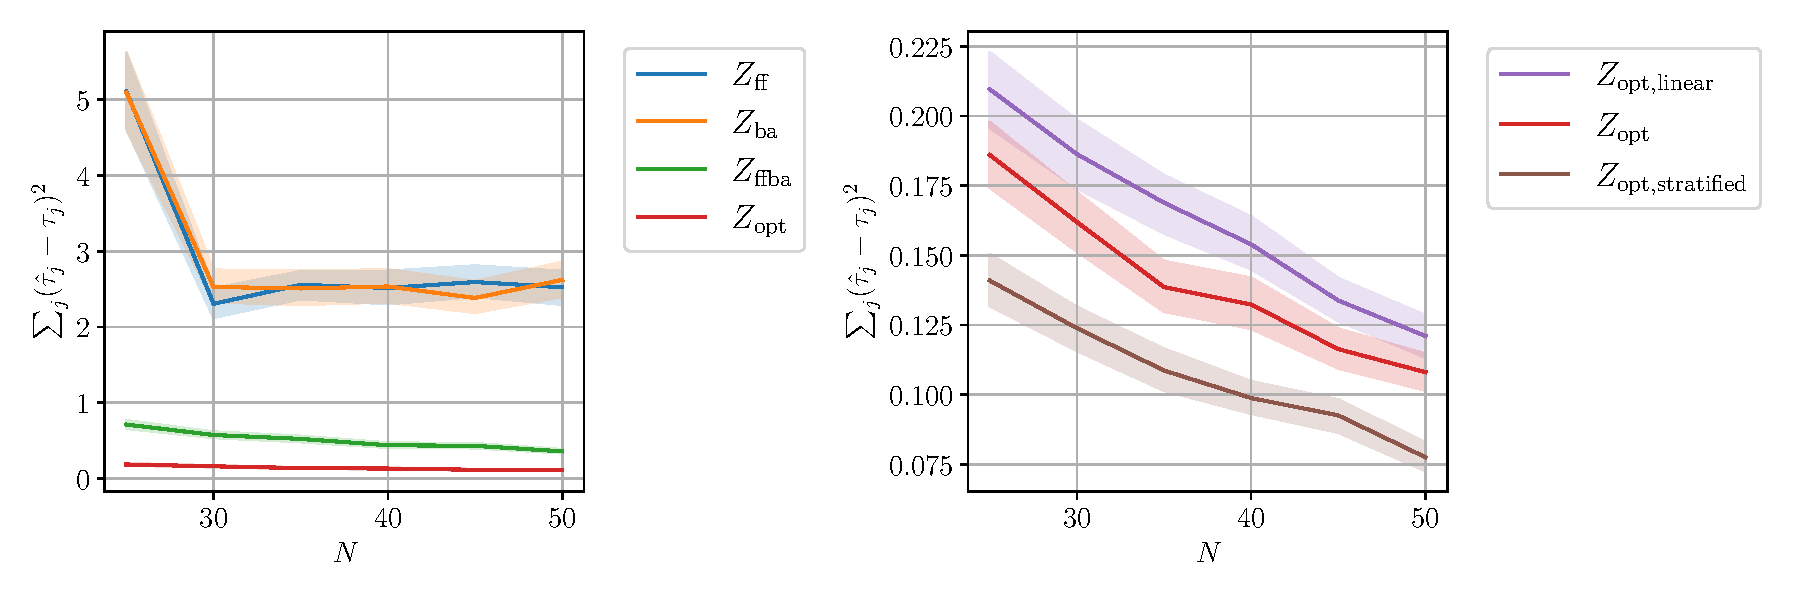
\includegraphics[width=1\linewidth]{plots/empirical/flu/nonadaptive/flu_T_7_varying_N_lag_2_agg.pdf}
	\end{subfigure}
	\caption{\textbf{Comparison of various designs in non-adaptive experiments.} These figures show the mean and 95\% confidence band of $\sum_{j}(\hat{\tau}_j - \tau_j)^2$ for various designs, based on 2,000 synthetic non-adaptive experiments with $\ell = 2$, $T = 7$ and varying $N$. The red curve in two figures are identical. The right figure zooms in the left one.
	}
	\label{fig:varying-N-flu}
\end{figure}

\paragraph{Stratification further improves upon the staggered treatment design.} The right subplot in Figure \ref{fig:varying-N-flu} additionally compares our nonlinear staggered designs \textit{without} stratification $Z_\OPT$ and \textit{with} stratification $Z_{\OPT,\mathrm{stratified}}$. 
Using $Z_{\OPT,\mathrm{stratified}}$ can further reduce 20\% samples to achieve the same total estimation error. 
Overall, this result suggests the existence of latent covariates in the original data. Therefore, when there are latent covariates, we could use the historical data that contains information about latent covariates to design a stratified experiment.  

\paragraph{Robustness to additional data sets.} Figure \ref{fig:additional-varying-N} in Section \ref{subsubsec:robustness-additional-data-set} shows that the above three findings continue to hold on the other three data sets, as $N$ is varied. Figure \ref{fig:additional-varying-T} in Section \ref{subsubsec:robustness-additional-data-set} shows the above three findings continue to hold on all four data sets, as $T$ is varied. 

{\blue 
\paragraph{Robustness to various specifications of the estimator.} 

We compare the performance of various treatment designs, as the model specification varies in Figure \ref{fig:various-estimation-method} in Section \ref{subsubsec:robustness-to-specification}. We show that the specification with $\alpha_i$, $\beta_t$, and $\*u_i$ significantly outperforms the specification where either $\alpha_i$, $\beta_t$, or $\*u_i$ is absent. Moreover, we show that $Z_{\OPT,\mathrm{stratified}}$ performs best under various specifications. Therefore, both the treatment decisions (design) and specification of the estimator play important roles in reducing the estimation error.}

 \paragraph{Robustness to other evaluation metrics.} The above three findings continue to hold when the evaluation metric is the squared estimation error of cumulative effect, as shown in Figure \ref{fig:varying-N-other-metrics} in Section \ref{subsubsec:robustness-to-alternative-metrics}. Figure \ref{fig:roc-equal-tau} in Section \ref{subsubsec:robustness-to-alternative-metrics} shows the ROC curve of various designs ({\it i.e.}, power vs. significance level), with AUC reported in Table \ref{tab:auc} in Section \ref{subsubsec:robustness-to-alternative-metrics}. Aligned with other metrics, $Z_{\OPT,\mathrm{stratified}}$ has consistently higher power than all other designs.



% \tocless
\subsection{Adaptive Experiments}\label{subsec:empirical-sequential}
In this section, we run synthetic adaptive experiments and evaluate adaptive designs produced by PGAE. We describe the experimental setup in Section \ref{subsec:sequential-setup} and then present the results in Section \ref{subsec:sequential-result}. We show the finite sample properties of Lemma \ref{lemma:asymptotic-tau-sigma} in Section \ref{subsec:finite-sample-lemma}. We also show the finite sample properties of Theorem 
\ref{theorem:asymptotic-page}  in Section \ref{subsec:finite-sample-pgae}\cmtfinal{, which implies the validity of the post-experiment inference using estimates produced by PGAE}.

% \tocless
\subsubsection{Setup}\label{subsec:sequential-setup}
\texttt{} \\
Suppose the adaptive experiment can run for a maximum of $T_{\max}$ periods in total and $\ell = 0$.\footnote{The results are robust to the hypothetical intervention with carryover effects, and are available upon request. } The adaptive experiment is terminated if the estimated precision is larger than threshold $c$. 

{\bf Treatment designs.} Overall, we consider the following three designs
\begin{enumerate}
    \item Adaptive design: The design produced by PGAE, with dimension $N \times \tilde{T}$\cmtfinal{, where $\tilde{T}$ is the actual termination time observed in the adaptive experiment}.
    \item Benchmark design: The initial design applied to $\mathcal{S}_{\fcs}$, $\mathcal{S}_{\ad,1}$, and $\mathcal{S}_{\ad,2}$ with dimension $N \times \tilde{T}$,  where for all $s\in[\tilde{T}]$,  $N^{-1} \sum_i z_{is} = \omega_{\mathrm{bm},s} = (2s - 1 - T_{\max})/{T_{\max}}$ which is optimal when $\tilde{T} = T_{\max}$ (identical to $Z_{\OPT, \mathrm{linear}}$ when $\tilde T = T_{\max}$). 
    \item Oracle design: The optimal design for a $\tilde{T}$-period experiment for $\mathcal{S}_{\fcs}$, $\mathcal{S}_{\ad,1}$, and $\mathcal{S}_{\ad,2}$ with dimension $N \times \tilde{T}$ and $N^{-1} \sum_i z_{is} = ({2s - 1- \tilde{T}})/{\tilde{T}}$ (identical to $Z_{\OPT, \mathrm{linear}}$ when $\tilde{T}$ is known ex ante).
\end{enumerate}

Note that the dimensionality of the three designs is the same, so we can make a fair comparison of the performance of these three designs.

{\bf Synthetic adaptive experimental data.} Similar to the synthetic non-adaptive experiments, we assume the original data does not contain any specific treatment that we study. Given a treatment design $Z$, the observed outcome for unit $i$ at time $s$ ($s \leq \tilde{T}$) is $Y_{is} = Y_{is}(-1) +  \tau_0  (z_{is} + 1)$.

\paragraph{Evaluation metrics.} As before, we randomly select $m$ blocks, each with dimension $N \times T_{\max}$ from the original control data. We report the mean and 95\% confidence band of $\big( \hat{\tau}^{(k)}_{0} - \tau_0 \big)^2$, where $\hat{\tau}^{(k)}_{0}$ is the estimated $\tau_0$ on the synthetic experimental data of dimension $N \times \tilde{T}^{(k)}$ based on the $k$-th block of the original data. $\tilde{T}^{(k)}$ is equal to the value of $\tilde{T}$ for that block; that is, $\tilde{T}$ can vary with $k$. 

% \tocless
\subsubsection{ Results}\label{subsec:sequential-result}
\texttt{}\\
{\blue 
We show an empirical distribution of the termination time $\tilde{T}$ in Figure \ref{fig:experiment-termination-time} and the estimation error of $\hat{\tau}_0$ of various designs in Figure \ref{fig:various-opt-design}. Four observations can be made from these figures.

First, PGAE indeed terminates the experiment early when precision exceeds the threshold. As shown Figure in \ref{fig:experiment-termination-time}, when $T_{\max} > 7$, the experiment is always terminated quite early ($\tilde{T}<T_{\max}/2$). This early stopping does not compromise the estimation error as Figure \ref{fig:various-opt-design} validates that the stopping rule works correctly and the estimation error of the adaptive design always stays below the variance threshold $1/c$. Looking at the results for different values of the threshold $c$, in Figure \ref{fig:experiment-termination-time} and Figure \ref{fig:experiment-termination-time-supp}, we see that the termination time tends to increase with the threshold, which is as expected.

Second, the adaptive design from PGAE consistently reduces the estimation error ({\it i.e.}, improves the precision) compared to the benchmark design ({\it i.e.}, non-adaptive design), where the benchmark design is used as initialization in PGAE. This implies that adaptive treatment decisions in PGAE can be useful in lowering the estimation error post-experiment. The reduction is more substantial for a larger $T_{\max}$. This is because when $T_{\max}$ is larger, the benchmark design is further away from the optimal design; hence there is more room for improvement for the adaptive design. The reduction is more than 20\% for $T_{\max} \geq 14$.


Third, the adaptive design consistently has a larger estimation error than the oracle design. The difference between adaptive and oracle designs is primarily due to the loss in precision from not knowing $\tilde{T}$ before the experiment starts. As the benchmark design differs from the oracle design and the treatment decisions are irreversible, the ``mistakes'' made in early time periods persistently continue to impact later periods. If we seek to narrow down the gap between adaptive and oracle designs, we can increase $N$, so that PGAE can learn the experiment termination time faster and make better treatment decisions early in the experiment.




    \begin{figure}[t!]
    \centering
    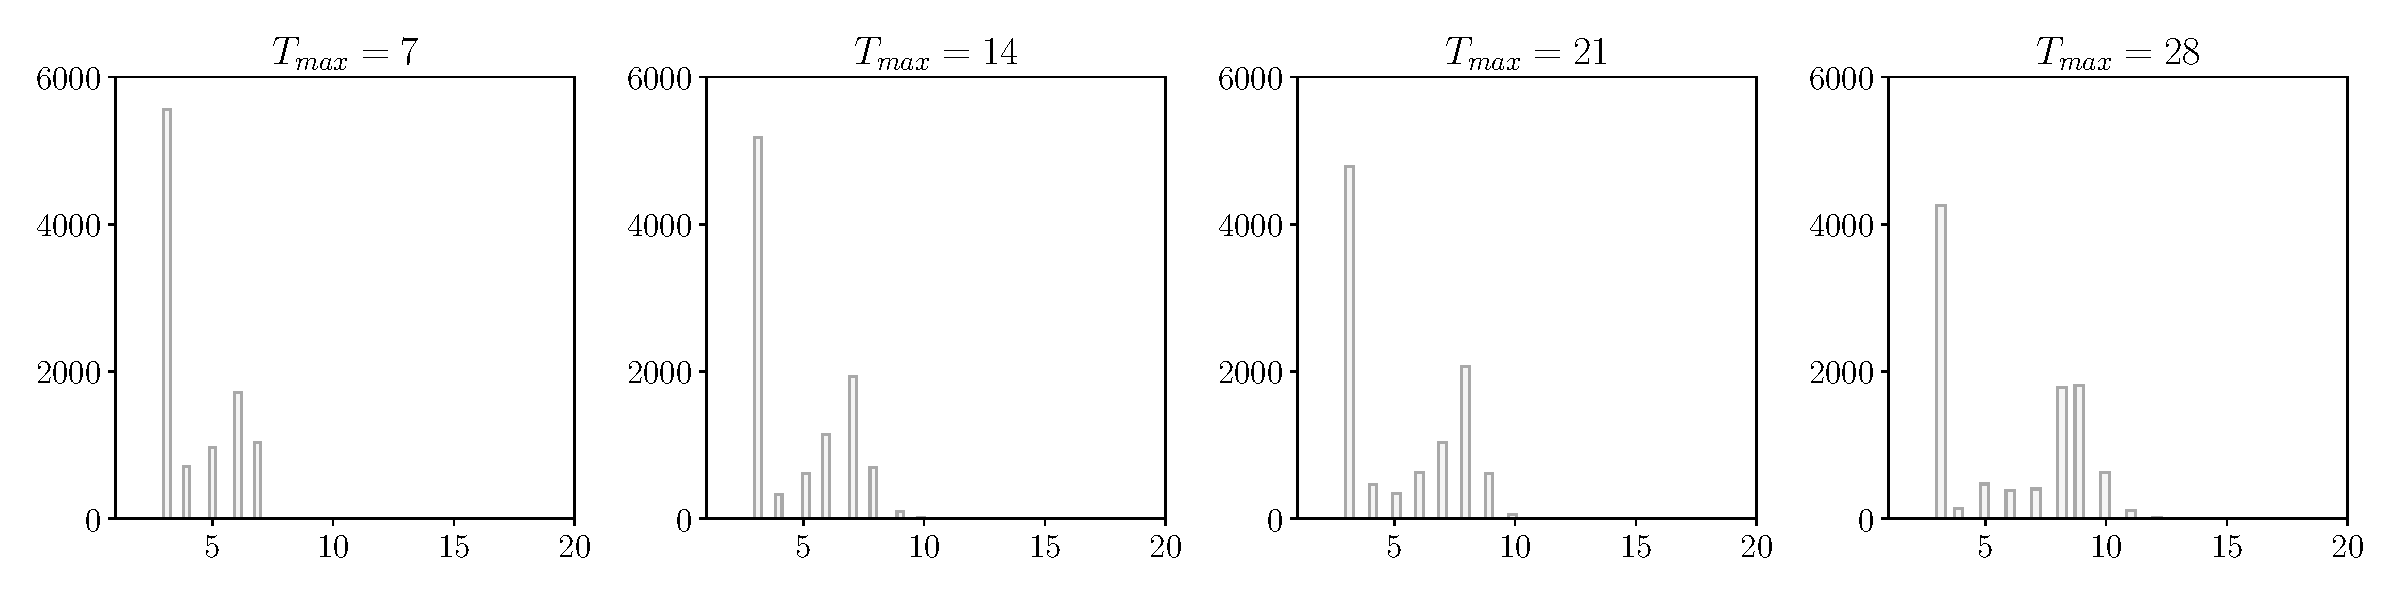
\includegraphics[width=1\linewidth]{plots/empirical/flu/adaptive/flu_termination_time.pdf}
	\caption{\textbf{Empirical distribution of termination time $\tilde{T}$ for various maximum duration.} This figure shows the histogram of the termination time $\tilde{T}$ for $T_{\max} \in \{7,14,21,28\}$ and $N=50$, based on 10,000 adaptive experiments. 
	In PGAE, NTU and each set of ATU have $10$ and $20$ units, respectively. $\tau_0$ is chosen at the minus 10\% of the average monthly flu occurrence rate, {\it i.e.}, $\tau_0 = -0.1 (NT_{\max})^{-1} \sum_{i,s} Y_{is}(-1)$. The experiment termination threshold is $c = 0.015 \cdot N/\tau_0^2 = 13.83$. The results in this figure are robust to the choice of $c$, as shown in Figure \ref{fig:experiment-termination-time-supp}.
	}
	\label{fig:experiment-termination-time}
\end{figure}



Finally, we note that there is a different trend in how the estimation error varies with $T_{\max}$ for different designs. For the benchmark design, the estimation error generally increases with $T_{\max}$. This is because as $T_{\max}$ increases, the benchmark design deviates more from the oracle design. For the oracle design, the estimation error consistently decreases with $T_{\max}$. This is because $\tilde{T}$ tends to increase with $T_{\max}$, as shown in Figure \ref{fig:experiment-termination-time}, and as a result, the precision of $\hat{\tau}_0$ using the oracle design increases with $\tilde{T}$.\footnote{The precision of $\hat{\tau}_0$ using the oracle design equals to $N (4\tilde{T}^2 - 1)/(3  \tilde T \sigma^2_\varepsilon) $, which increases with $\tilde{T}$.} For the adaptive design, since the algorithm stops as the estimated precision reaches the fixed threshold $c$, we expect the estimation error to generally stay flat for various $T_{\max}$. But since the precision estimation is not exact, and is actually a conservative one, there is no specific pattern for fluctuations in the estimation error.
    \begin{figure}[t!]
    \centering
    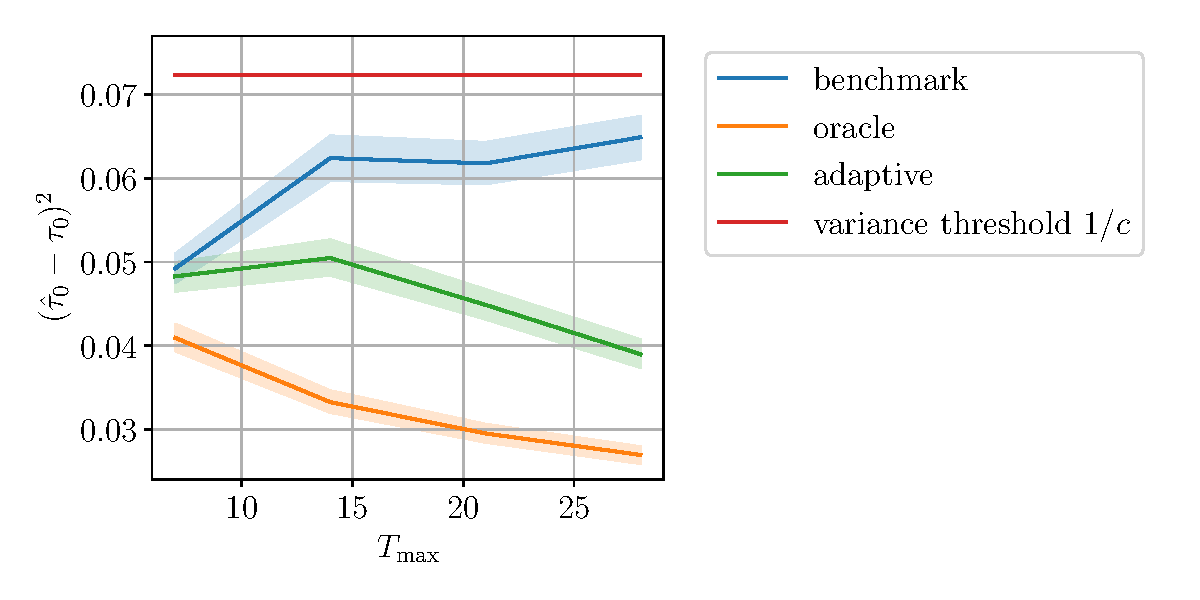
\includegraphics[width=0.6\linewidth]{plots/empirical/flu/adaptive/flu_adaptive_comparison.pdf}
	\caption{\textbf{Comparison of various designs in adaptive experiments.} This figure shows the mean and 95\% confidence band of $(\hat{\tau}_0 - \tau_0)^2$ for adaptive, benchmark, and oracle designs, based on 10,000 synthetic adaptive experiments. As the precision threshold is $c = 13.83$, the corresponding variance threshold $\var(\hat{\tau})$ is $1/c=0.072$. 
	The results in this figure are robust to the choice of $c$, as shown in Figure \ref{fig:experiment-termination-time-supp}.
	}
	\label{fig:various-opt-design}
\end{figure}


}